\documentclass[10pt]{article}
% pdfTeX hashes this string into the trailer /ID, so a single shared value
% would give the anonymous and archival PDFs an identical, trivially
% cross-referenced identifier.  Each build therefore seeds a distinct one.
\ifdefined\ARXIVVERSION
  \pdftrailerid{kaetram-tool-routing-archival-build}
\else
  \pdftrailerid{kaetram-tool-routing-review-build}
\fi
\ifdefined\ARXIVVERSION
  \usepackage[preprint]{tmlr}
\else
  \usepackage{tmlr}
  % Generated locally from the anonymous review projections. This file is
  % intentionally untracked and contains no public-fork fingerprints.
  \input{review-roots.tex}
\fi
\usepackage{amsmath,amssymb,booktabs,array,multirow}
\usepackage{graphicx}
\usepackage{xcolor}
\usepackage{float}
\usepackage{needspace}
\usepackage{tikz}
\usepackage{pgfplots}
\usetikzlibrary{arrows.meta,positioning,calc}
\pgfplotsset{compat=1.18}
\usepackage{hyperref}
\usepackage{url}
\ifdefined\ARXIVVERSION
  \hypersetup{
    hidelinks,
    pdftitle={\ArchivePDFTitle},
    pdfauthor={\ArchivePDFAuthor}
  }
\else
  \hypersetup{hidelinks}
\fi

\title{Stranded in Reasoning: Auditing Where Tool Calls Stop in a Persistent
Language-Model Agent\thanks{Large language models materially assisted literature
search, code review, experimental-design critique, and manuscript drafting.
The human authors verified the evidence, analyses, citations, and final claims
and retain full responsibility for the work.}}

\ifdefined\ARXIVVERSION
  \author{\ArchiveAuthorBlock}
\else
  % Author identities are suppressed by the review-mode TMLR style.
  \author{Anonymous authors}
\fi

\def\month{MM}
\def\year{YYYY}
\def\openreview{\url{https://openreview.net/forum?id=XXXX}}

\newcommand{\opd}{\textsc{opd}}
\newcommand{\core}{\textsc{Core-3}}
\newcommand{\pp}{\,pp}
% Generated by scripts/opd/render_tmlr_figures.py; do not edit.
\newcommand{\RecoveryRawGenerations}{958}
\newcommand{\RecoveryEligibleGenerations}{0}
\newcommand{\VOneSeedGroups}{240}
\newcommand{\VOneDiverseSeedGroups}{0}
\newcommand{\VTwoSuccessfulRequests}{1200}
\newcommand{\VThreeSuccessfulRequests}{1200}
\newcommand{\RoutingVTwoProtocolValid}{9}
\newcommand{\RoutingVTwoFullPass}{0}
\newcommand{\RoutingVThreeProtocolValid}{9}
\newcommand{\RoutingVThreeFullPass}{9}
\newcommand{\VTwoBaseEffect}{23}
\newcommand{\VTwoBasePositive}{14}
\newcommand{\VTwoBaseZero}{5}
\newcommand{\VTwoBaseNegative}{1}
\newcommand{\VTwoBaseValidAnyEffect}{37}
\newcommand{\VTwoRoundTwoEffect}{13}
\newcommand{\VTwoRoundTwoPositive}{12}
\newcommand{\VTwoRoundTwoZero}{6}
\newcommand{\VTwoRoundTwoNegative}{2}
\newcommand{\VTwoRoundTwoValidAnyEffect}{16.5}
\newcommand{\VTwoRoundThreeEffect}{10}
\newcommand{\VTwoRoundThreePositive}{13}
\newcommand{\VTwoRoundThreeZero}{4}
\newcommand{\VTwoRoundThreeNegative}{3}
\newcommand{\VTwoRoundThreeValidAnyEffect}{19}
\newcommand{\VThreeBaseEffect}{13}
\newcommand{\VThreeBasePositive}{11}
\newcommand{\VThreeBaseZero}{7}
\newcommand{\VThreeBaseNegative}{2}
\newcommand{\VThreeBaseValidAnyEffect}{24}
\newcommand{\VThreeRoundTwoEffect}{5.5}
\newcommand{\VThreeRoundTwoPositive}{7}
\newcommand{\VThreeRoundTwoZero}{8}
\newcommand{\VThreeRoundTwoNegative}{5}
\newcommand{\VThreeRoundTwoValidAnyEffect}{25}
\newcommand{\VThreeRoundThreeEffect}{9}
\newcommand{\VThreeRoundThreePositive}{9}
\newcommand{\VThreeRoundThreeZero}{10}
\newcommand{\VThreeRoundThreeNegative}{1}
\newcommand{\VThreeRoundThreeValidAnyEffect}{31.5}

% Publication figures. Numerical macros come from the evidence-bound
% figure-data.tex file generated from released analyses.
\definecolor{routeblue}{HTML}{2B6CB0}
\definecolor{routeorange}{HTML}{DD6B20}
\definecolor{routegreen}{HTML}{2F855A}
\definecolor{routered}{HTML}{C53030}
\definecolor{routegray}{HTML}{718096}
\definecolor{routeink}{HTML}{2D3748}

\newcommand{\AuditOverviewFigure}{%
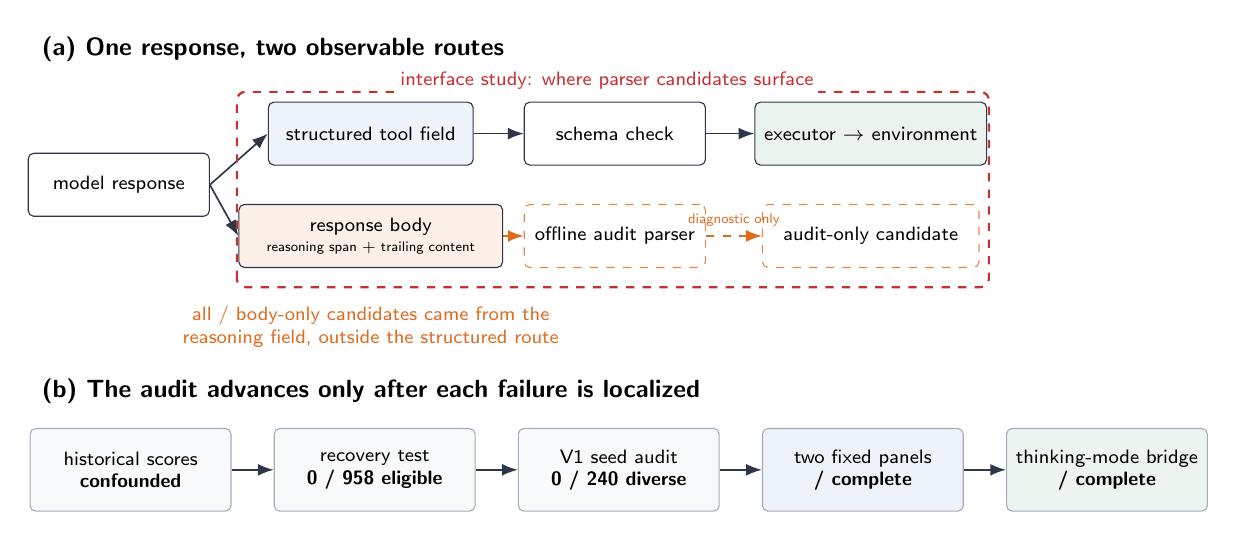
\begin{tikzpicture}[
  font=\sffamily\scriptsize,
  line/.style={-{Latex[length=2mm]},semithick,draw=routeink},
  box/.style={draw=routeink,rounded corners=2pt,align=center,minimum height=8mm,fill=white},
  stage/.style={draw=routegray!65,rounded corners=2pt,align=center,minimum width=2.55cm,
                minimum height=1.05cm,fill=routegray!5},
]
  \node[font=\sffamily\bfseries\small,anchor=west] at (-0.3,1.72)
    {(a) One response, two observable routes};
  \node[box,minimum width=2.3cm] (model) at (0.8,0) {model response};
  \node[box,minimum width=2.6cm,fill=routeblue!8] (structured) at (4.0,0.65)
    {structured tool field};
  \node[box,minimum width=3.35cm,fill=routeorange!10,align=center,inner sep=3pt] (content) at (4.0,-0.65)
    {response body\\[-1pt]{\fontsize{5.2}{6}\selectfont reasoning span $+$ trailing content}};
  \node[box,minimum width=2.3cm] (schema) at (7.1,0.65) {schema check};
  \node[box,minimum width=2.3cm,draw=routeorange!80,dashed] (parser) at (7.1,-0.65) {offline audit parser};
  \node[box,minimum width=2.75cm,fill=routegreen!10] (executor) at (10.35,0.65)
    {executor $\rightarrow$ environment};
  \node[box,minimum width=2.75cm,draw=routeorange!80,dashed] (candidate) at (10.35,-0.65)
    {audit-only candidate};
  \draw[line] (model.east) -- (structured.west);
  \draw[line] (model.east) -- (content.west);
  \draw[line] (structured) -- (schema);
  \draw[line,routeorange,dashed] (content) -- (parser);
  \draw[line] (schema.east) -- (executor.west);
  \draw[line,routeorange,dashed] (parser.east) -- node[above,font=\sffamily\tiny] {diagnostic only} (candidate.west);
  \draw[routered,dashed,rounded corners=3pt,thick]
    (2.30,-1.30) rectangle (11.85,1.18);
  \node[routered,fill=white,inner sep=1.5pt,anchor=south] at (7.0,1.15)
    {interface study: where parser candidates surface};
  \node[routeorange,align=center,anchor=north,font=\sffamily\scriptsize] at (4.0,-1.42)
    {all \SpanInsideReasoning{}/\SpanRecoveredCalls{} body-only candidates came from the\\reasoning field, outside the structured route};

  \node[font=\sffamily\bfseries\small,anchor=west] at (-0.3,-2.62)
    {(b) The audit advances only after each failure is localized};
  \node[stage] (s1) at (0.95,-3.62) {historical scores\\\textbf{confounded}};
  \node[stage] (s2) at (4.05,-3.62) {recovery test\\\textbf{\RecoveryEligibleGenerations{} / \RecoveryRawGenerations{} eligible}};
  \node[stage] (s3) at (7.15,-3.62) {V1 seed audit\\\textbf{\VOneDiverseSeedGroups{} / \VOneSeedGroups{} diverse}};
  \node[stage,fill=routeblue!8] (s4) at (10.25,-3.62) {two fixed panels\\\textbf{\SpanTotalRows{}/\SpanTotalRows{} complete}};
  \node[stage,fill=routegreen!9] (s5) at (13.35,-3.62) {thinking-mode bridge\\\textbf{\ParityPooledRequests{}/\ParityPooledRequests{} complete}};
  \draw[line] (s1) -- (s2);
  \draw[line] (s2) -- (s3);
  \draw[line] (s3) -- (s4);
  \draw[line] (s4) -- (s5);
\end{tikzpicture}%
}

\newcommand{\ServingRegimeParityFigure}{%
\begin{tikzpicture}[font=\sffamily\scriptsize]
  \begin{axis}[
    name=parityroutes,
    width=9.15cm,height=6.15cm,
    title style={font=\sffamily\bfseries\small,align=center,yshift=3.2ex},
    title={(a) Where action candidates surface},
    xbar stacked,
    xmin=0,xmax=\ParityRequestsPerCheckpoint,
    xtick={0,\ParityQuarterRequests,\ParityHalfRequests,\ParityThreeQuarterRequests,\ParityRequestsPerCheckpoint},
    xlabel={matched request cells (each bar totals \ParityRequestsPerCheckpoint)},
    ytick={1,2,3,4,5,6},
    yticklabels={Round 3 / off,Round 3 / on,Round 2 / off,Round 2 / on,Base / off,Base / on},
    bar width=7pt,
    axis line style={routegray!65},
    xmajorgrids,grid style={routegray!18},
    tick label style={font=\sffamily\scriptsize},
    label style={font=\sffamily\scriptsize},
    legend style={draw=none,font=\sffamily\scriptsize,at={(0.5,1.03)},anchor=south,legend columns=3},
  ]
    \addplot+[fill=routeblue,draw=white] coordinates {
      (\ParityRoundThreeThinkingOffStructuredCount,1)
      (\ParityRoundThreeThinkingOnStructuredCount,2)
      (\ParityRoundTwoThinkingOffStructuredCount,3)
      (\ParityRoundTwoThinkingOnStructuredCount,4)
      (\ParityBaseThinkingOffStructuredCount,5)
      (\ParityBaseThinkingOnStructuredCount,6)};
    \addlegendentry{structured call}
    \addplot+[fill=routeorange,draw=white] coordinates {
      (\ParityRoundThreeThinkingOffBodyOnlyCount,1)
      (\ParityRoundThreeThinkingOnBodyOnlyCount,2)
      (\ParityRoundTwoThinkingOffBodyOnlyCount,3)
      (\ParityRoundTwoThinkingOnBodyOnlyCount,4)
      (\ParityBaseThinkingOffBodyOnlyCount,5)
      (\ParityBaseThinkingOnBodyOnlyCount,6)};
    \addlegendentry{body-only candidate}
    \addplot+[fill=routegray!45,draw=white] coordinates {
      (\ParityRoundThreeThinkingOffNoCandidateCount,1)
      (\ParityRoundThreeThinkingOnNoCandidateCount,2)
      (\ParityRoundTwoThinkingOffNoCandidateCount,3)
      (\ParityRoundTwoThinkingOnNoCandidateCount,4)
      (\ParityBaseThinkingOffNoCandidateCount,5)
      (\ParityBaseThinkingOnNoCandidateCount,6)};
    \addlegendentry{no parseable call}
    \draw[routegray!55,thin] (axis cs:0,2.5) --
      (axis cs:\ParityRequestsPerCheckpoint,2.5);
    \draw[routegray!55,thin] (axis cs:0,4.5) --
      (axis cs:\ParityRequestsPerCheckpoint,4.5);
  \end{axis}

  \begin{axis}[
    at={(9.65cm,0)},anchor=south west,
    width=5.85cm,height=6.15cm,
    title style={font=\sffamily\bfseries\small,align=center,yshift=3.2ex},
    title={(b) Change when thinking is off},
    xlabel={off $-$ on (percentage points)},
    ytick={1,2,3},yticklabels={Round 3,Round 2,Base},
    ymin=.65,ymax=3.35,
    xmajorgrids,grid style={routegray!18},
    axis line style={routegray!65},
    enlarge x limits=0.18,
    tick label style={font=\sffamily\scriptsize},
    label style={font=\sffamily\scriptsize},
    legend style={draw=none,font=\sffamily\scriptsize,at={(0.5,1.03)},anchor=south,legend columns=2},
  ]
    \addplot+[draw=none,mark=none,forget plot] coordinates {(0,1)};
    \addplot+[dashed,routegray,mark=none,forget plot] coordinates {(0,.65) (0,3.35)};
    \addplot+[only marks,mark=*,mark size=2.4pt,color=routeorange,
              nodes near coords,point meta=x,
              every node near coord/.append style={font=\sffamily\tiny,anchor=south}]
      coordinates {(\ParityRoundThreeBodyOnlyDeltaPP,1.10)
                   (\ParityRoundTwoBodyOnlyDeltaPP,2.10)
                   (\ParityBaseBodyOnlyDeltaPP,3.10)};
    \addlegendentry{body-only candidate}
    \addplot+[only marks,mark=square*,mark size=2.2pt,color=routeblue,
              nodes near coords,point meta=x,
              every node near coord/.append style={font=\sffamily\tiny,anchor=north}]
      coordinates {(\ParityRoundThreeStructuredDeltaPP,.90)
                   (\ParityRoundTwoStructuredDeltaPP,1.90)
                   (\ParityBaseStructuredDeltaPP,2.90)};
    \addlegendentry{structured call}
  \end{axis}
\end{tikzpicture}%
}

\newcommand{\PrimaryResultsFigure}{%
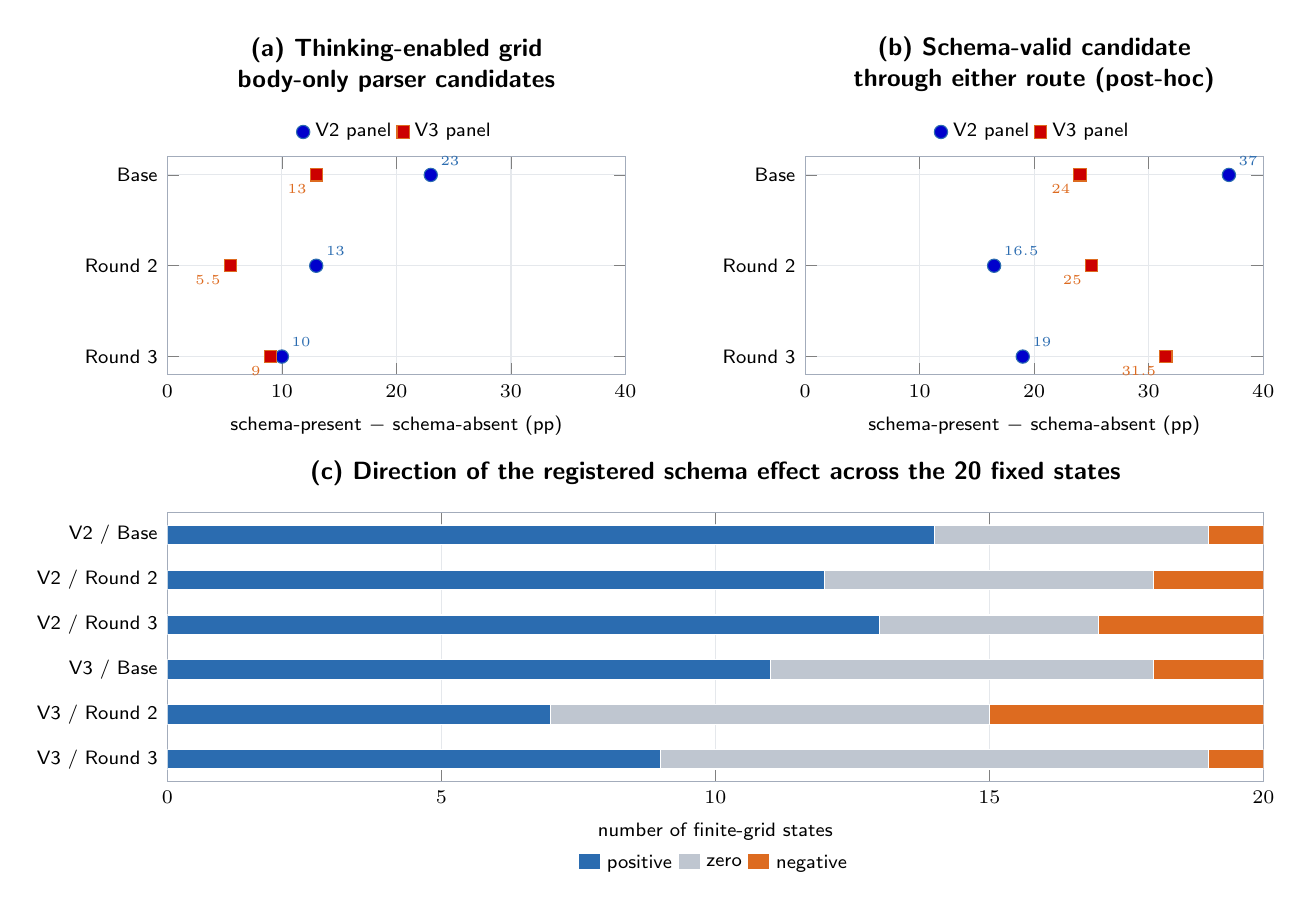
\begin{tikzpicture}[font=\sffamily\scriptsize]
  \begin{axis}[
    name=primary,
    width=7.4cm,height=4.35cm,
    title style={font=\sffamily\bfseries\small,align=center,yshift=3.2ex},
    title={(a) Thinking-enabled grid\\body-only parser candidates},
    xmin=0,xmax=40,xtick={0,10,20,30,40},
    xlabel={schema-present $-$ schema-absent (pp)},
    ytick={1,2,3},yticklabels={Round 3,Round 2,Base},
    grid=major,grid style={routegray!18},axis line style={routegray!65},
    tick label style={font=\sffamily\scriptsize},label style={font=\sffamily\scriptsize},
    legend style={draw=none,font=\sffamily\scriptsize,at={(0.5,1.02)},anchor=south,legend columns=2},
  ]
    \addplot+[only marks,mark=*,mark size=2.4pt,color=routeblue,nodes near coords,
              point meta=x,every node near coord/.append style={font=\sffamily\tiny,anchor=south west}]
      coordinates {(\VTwoRoundThreeEffect,1) (\VTwoRoundTwoEffect,2) (\VTwoBaseEffect,3)};
    \addlegendentry{V2 panel}
    \addplot+[only marks,mark=square*,mark size=2.2pt,color=routeorange,nodes near coords,
              point meta=x,every node near coord/.append style={font=\sffamily\tiny,anchor=north east}]
      coordinates {(\VThreeRoundThreeEffect,1) (\VThreeRoundTwoEffect,2) (\VThreeBaseEffect,3)};
    \addlegendentry{V3 panel}
  \end{axis}

  \begin{axis}[
    at={(8.1cm,0)},anchor=south west,
    width=7.4cm,height=4.35cm,
    title style={font=\sffamily\bfseries\small,align=center,yshift=3.2ex},
    title={(b) Schema-valid candidate\\through either route (post-hoc)},
    xmin=0,xmax=40,xtick={0,10,20,30,40},
    xlabel={schema-present $-$ schema-absent (pp)},
    ytick={1,2,3},yticklabels={Round 3,Round 2,Base},
    grid=major,grid style={routegray!18},axis line style={routegray!65},
    tick label style={font=\sffamily\scriptsize},label style={font=\sffamily\scriptsize},
    legend style={draw=none,font=\sffamily\scriptsize,at={(0.5,1.02)},anchor=south,legend columns=2},
  ]
    \addplot+[only marks,mark=*,mark size=2.4pt,color=routeblue,nodes near coords,
              point meta=x,every node near coord/.append style={font=\sffamily\tiny,anchor=south west}]
      coordinates {(\VTwoRoundThreeValidAnyEffect,1) (\VTwoRoundTwoValidAnyEffect,2) (\VTwoBaseValidAnyEffect,3)};
    \addlegendentry{V2 panel}
    \addplot+[only marks,mark=square*,mark size=2.2pt,color=routeorange,nodes near coords,
              point meta=x,every node near coord/.append style={font=\sffamily\tiny,anchor=north east}]
      coordinates {(\VThreeRoundThreeValidAnyEffect,1) (\VThreeRoundTwoValidAnyEffect,2) (\VThreeBaseValidAnyEffect,3)};
    \addlegendentry{V3 panel}
  \end{axis}

  \begin{axis}[
    at={(0,-1.75cm)},anchor=north west,
    width=15.5cm,height=5.0cm,
    title style={font=\sffamily\bfseries\small},
    title={(c) Direction of the registered schema effect across the 20 fixed states},
    xbar stacked,xmin=0,xmax=20,xtick={0,5,10,15,20},
    xlabel={number of finite-grid states},
    ytick={1,2,3,4,5,6},
    yticklabels={V3 / Round 3,V3 / Round 2,V3 / Base,V2 / Round 3,V2 / Round 2,V2 / Base},
    bar width=7pt,
    axis line style={routegray!65},grid=major,grid style={routegray!18},
    tick label style={font=\sffamily\scriptsize},label style={font=\sffamily\scriptsize},
    legend style={draw=none,font=\sffamily\scriptsize,at={(0.5,-0.23)},anchor=north,legend columns=3},
  ]
    \addplot+[fill=routeblue,draw=white] coordinates {
      (\VThreeRoundThreePositive,1) (\VThreeRoundTwoPositive,2) (\VThreeBasePositive,3)
      (\VTwoRoundThreePositive,4) (\VTwoRoundTwoPositive,5) (\VTwoBasePositive,6)};
    \addlegendentry{positive}
    \addplot+[fill=routegray!45,draw=white] coordinates {
      (\VThreeRoundThreeZero,1) (\VThreeRoundTwoZero,2) (\VThreeBaseZero,3)
      (\VTwoRoundThreeZero,4) (\VTwoRoundTwoZero,5) (\VTwoBaseZero,6)};
    \addlegendentry{zero}
    \addplot+[fill=routeorange,draw=white] coordinates {
      (\VThreeRoundThreeNegative,1) (\VThreeRoundTwoNegative,2) (\VThreeBaseNegative,3)
      (\VTwoRoundThreeNegative,4) (\VTwoRoundTwoNegative,5) (\VTwoBaseNegative,6)};
    \addlegendentry{negative}
  \end{axis}
\end{tikzpicture}%
}

\newcommand{\MeasurementRepairFigure}{%
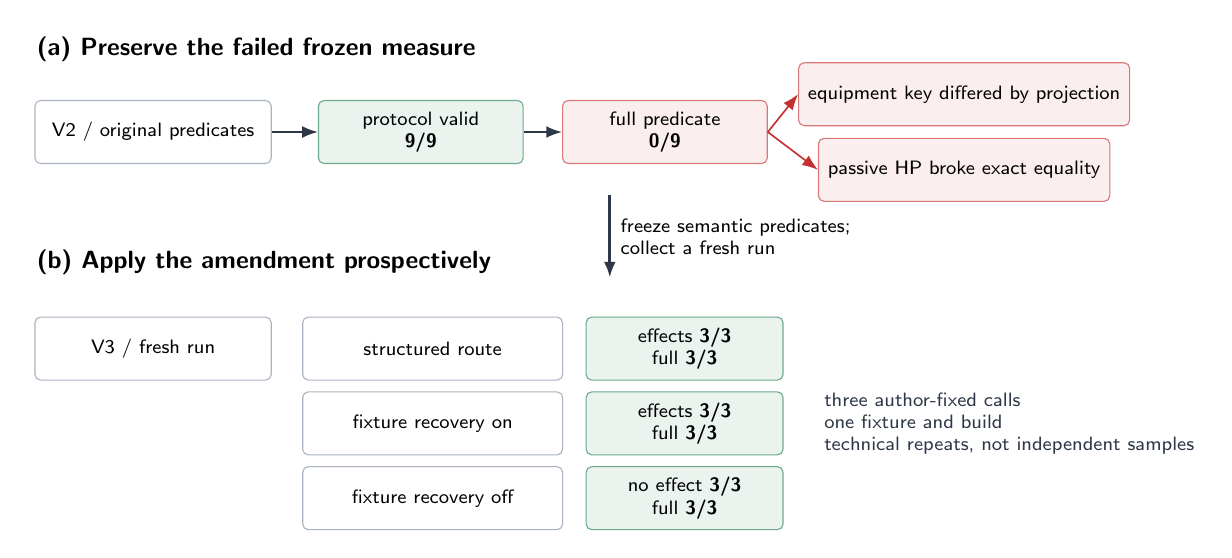
\begin{tikzpicture}[
  font=\sffamily\scriptsize,
  line/.style={-{Latex[length=2mm]},semithick,draw=routeink},
  cell/.style={draw=routegray!60,rounded corners=2pt,align=center,minimum height=8mm},
  good/.style={cell,fill=routegreen!10,draw=routegreen!70},
  bad/.style={cell,fill=routered!8,draw=routered!65},
]
  \node[font=\sffamily\bfseries\small,anchor=west] at (0,1.05)
    {(a) Preserve the failed frozen measure};
  \node[cell,minimum width=3.0cm] (v2) at (1.6,0) {V2 / original predicates};
  \node[good,minimum width=2.6cm] (v2p) at (5.0,0) {protocol valid\\\textbf{\RoutingVTwoProtocolValid/9}};
  \node[bad,minimum width=2.6cm] (v2f) at (8.1,0) {full predicate\\\textbf{\RoutingVTwoFullPass/9}};
  \draw[line] (v2) -- (v2p); \draw[line] (v2p) -- (v2f);
  \node[bad,minimum width=3.7cm] (d1) at (11.9,0.48) {equipment key differed by projection};
  \node[bad,minimum width=3.7cm] (d2) at (11.9,-0.48) {passive HP broke exact equality};
  \draw[line,routered] (v2f.east) -- (d1.west);
  \draw[line,routered] (v2f.east) -- (d2.west);

  \draw[line,very thick] (7.4,-0.8) -- node[right,align=left] {freeze semantic predicates;\\collect a fresh run} (7.4,-1.85);
  \node[font=\sffamily\bfseries\small,anchor=west] at (0,-1.65)
    {(b) Apply the amendment prospectively};
  \node[cell,minimum width=3.0cm] at (1.6,-2.75) {V3 / fresh run};
  \node[cell,minimum width=3.3cm] at (5.15,-2.75) {structured route};
  \node[good,minimum width=2.5cm] at (8.35,-2.75) {effects \textbf{3/3}\\full \textbf{3/3}};
  \node[cell,minimum width=3.3cm] at (5.15,-3.70) {fixture recovery on};
  \node[good,minimum width=2.5cm] at (8.35,-3.70) {effects \textbf{3/3}\\full \textbf{3/3}};
  \node[cell,minimum width=3.3cm] at (5.15,-4.65) {fixture recovery off};
  \node[good,minimum width=2.5cm] at (8.35,-4.65) {no effect \textbf{3/3}\\full \textbf{3/3}};
  \node[align=left,anchor=west,text=routeink] at (10.0,-3.70)
    {three author-fixed calls\\one fixture and build\\technical repeats, not independent samples};
\end{tikzpicture}%
}


\begin{document}
\maketitle

\begin{abstract}
A tool-using language-model agent can write a well-formed action and still
change nothing, because the action never leaves the channel it was written in.
We audit this failure in a 2B agent controlling a persistent game through 17
typed tools. Historical scores could not identify a training effect because
weights, states, interfaces, and runtime recovery changed together. A
prospective 18-condition test then found that recovery was never eligible to act
in 958 generations. We therefore isolated the model-visible interface. A
discovery study revealed that nominal request seeds produced duplicate outputs.
After repairing sampling, a frozen 1,200-request study evaluated three
checkpoints on 20 previously unseen decision states with five effective seeds.
Supplying the 17-tool schema through the endpoint's structured tools field
increased parser-recoverable calls that were absent from the structured field
by +23, +13, and +10 percentage points. Repeating the same protocol on a
different retained state set produced +13, +5.5, and +9 points; no source log or
rendered model input overlapped the first study. This second panel is a
robustness check, not independent replication. Crucially, a post-outcome
localization shows that all \SpanRecoveredCalls{} such calls across both panels
sit inside the model's reasoning span, and that only
\SpanRowsWithTrailingText{} of \SpanTotalRows{} responses carry any
post-reasoning content at all. The agent is therefore not losing actions to a careless executor: it is
writing them where a correct executor should decline to read. Post-hoc analyses
on both panels found more schema-valid candidates through either route. Finally,
a model-free diagnostic preserved a failed measurement, amended it
prospectively, and on a fresh run routed all three frozen calls in each of six
active-route trials while the three disabled-control trials showed no registered
action effect. The contribution is a reviewer-recomputable audit of where
actions stop between model and environment---not a checkpoint ranking, recovery
benefit, broad generalization, or training effect.
\end{abstract}

\section{Introduction}

Tool use is often reported as though it were a property of model weights. In a
deployed agent, however, an action must survive a chain of contracts. The model
sees a rendered description of available tools, emits both text and structured
fields, an endpoint serializes those fields, a parser accepts or rejects them,
and a harness may rewrite or recover content before an environment changes
state. A valid command at one layer can be invisible at the next.

This distinction matters most in long-horizon settings. If a command is silently
dropped, the agent receives no state transition, later observations diverge,
and an eventual task score attributes the failure to the entire policy. If
model weights, prompts, schemas, parsers, and recovery rules also change between
runs, the score does not reveal which component helped or failed. The resulting
ambiguity is not fixed by collecting more turns from the same run.

We encountered this problem while auditing a small language-model agent in a
persistent MMORPG. The agent receives a procedural quest guide and acts through
17 typed tools. Historical development records suggested that changing the
training-state distribution improved quest progress, while later runs also
changed the tool interface and runtime recovery. The records preserved exact
descriptive scores, but not the exact checkpoint, environment reset,
model-visible prompt, or random seed for every run. Rather than treat those
scores as causal evidence, we used them to identify a mechanism that could be
tested directly.

The resulting study follows a sequence that is useful beyond this game. First,
we tied every historical claim to retained evidence and marked the comparisons
that could not identify an effect. Second, we ran a prospective recovery
factorial and checked
whether the intervention actually fired. It did not: none of 958 generations
was eligible. Third, a registered fixed-state grid isolated two model-visible
interface factors and exposed recoverable calls that were written into the
response body rather than delivered through the structured channel. Fourth, an audit discovered
that nominal request seeds had not changed sampling. We repaired the seed path
and prospectively froze an outcome-unseen confirmation instead of retrospectively
upgrading the first study. Finally, we repeated the unchanged grid on a
different retained state panel and followed three frozen calls across the next
execution boundary with a prospectively repaired measure.

\begin{figure}[t]
\centering
\AuditOverviewFigure
\caption{The audit separates response routing from downstream execution and
advances only after each failed check is localized. A call written into the
response body is not visible to an executor that reads only the structured
field; Section~\ref{sec:where-calls-sit} shows that in this study every such
call was written inside the model's reasoning span, where a correct executor
should decline to read it. Numbers are regenerated from the released public
summaries.}
\label{fig:routing}
\end{figure}

Our contributions are:

\begin{enumerate}
  \item We decompose tool execution into a model-to-environment routing contract
  and define auditable outcomes that distinguish a structured envelope, a
  parser-recoverable call in the response body, a malformed surface form, and no
  recoverable call.
  \item We report a registered outcome-unseen finite-grid confirmation across
  three fixed checkpoints and a non-confirmatory extension on a different
  retained panel. Native schema exposure increased content-only
  recoverable-call incidence at every checkpoint on both panels, with effects
  of 10--23 and 5.5--13 percentage points.
  \item We localize where those calls actually sit. All \SpanRecoveredCalls{}
  recovered calls across both panels lie inside the model's reasoning span, and
  only \SpanRowsWithTrailingText{} of \SpanTotalRows{}
  responses contain any text after that span closes. The failure is therefore
  not a permissive parser meeting a strict executor; it is a model that never
  exits its reasoning channel to emit the action. This reframes recovery from a
  missed opportunity into a hazard.
  \item We provide a failure-aware, reviewer-recomputable evidence sequence that
  preserves failed manipulation, effective-seed, and measurement checks. After
  prospective measurement repair, three author-fixed calls produced their
  registered fixture effects in all six active-route trials, while the disabled
  arm showed no registered action effect in 3/3.
\end{enumerate}

The bounded conclusion is about this action-routing contract. The three
checkpoints form one model lineage, both state panels come from the same project
and evaluation regime, and the renderer is fixed. We do not treat checkpoints
as training replicates, call the two panels independent replications, infer a
recovery benefit, or claim improved quest performance.

\section{Setting and Action-Routing Contract}

\subsection{Persistent tool-use setting}

The environment is a permissioned fork of the open-source Kaetram MMORPG
\citep{kaetram2026}. A Qwen/Qwen3.5-2B agent \citep{qwen35modelcards2026}
controls a persistent player through 17 tools for observation, navigation,
combat, gathering, dialogue, quest inspection, inventory use, and crafting.
Game state persists across conversation rollovers. The system prompt contains
procedural quest guidance, so the benchmark measures execution of a supplied
plan rather than autonomous discovery of game rules.

The historical development score, \core{}, counts newly reached stages in
three quest chains, with ten stages per agent and three prompt variants for a
maximum of 30. This score is useful for end-to-end development, much like
persistent state metrics in $\tau$-bench \citep{yao2025taubench}, but it is too
coarse to localize a dropped action. The registered interface studies therefore
operate on fixed historical decision states and inspect the immediate model
response.

\subsection{How a recoverable action can disappear}

Figure~\ref{fig:routing} separates the layers between a model-visible tool and
an environment transition. The registered ``native schema'' treatment means
that a hash-bound 17-tool schema is supplied through the model endpoint's
native \texttt{tools} field. It is not claimed to be byte-identical to every
historical production schema.

For example, a response may contain a canonical function block naming
\texttt{navigate} with valid JSON-like arguments, while its structured
\texttt{tool\_calls} field is empty. The harness sees only response body text
unless an explicit recovery layer parses that block. We use the following
taxonomy:

\begin{description}
  \item[Structured envelope.] The endpoint returns at least one call in the
  structured field. Schema validity is a separate question.
  \item[Content-only recoverable call.] The structured field is empty, but the
  prospectively frozen deterministic parser recovers at least one candidate from the
  response content. This is the primary outcome, also called a recovery
  opportunity. ``Content'' here names the response \texttt{content} field as the
  endpoint returns it. Section~\ref{sec:reasoning-regime} shows that in this
  serving regime that field is dominated by the model's reasoning span, and
  Section~\ref{sec:where-calls-sit} shows that every recovered call in this study
  lies inside it. We retain the registered label because it is frozen in the
  released artifacts, but it should not be read as ``ordinary prose addressed to
  the user.''
  \item[No recoverable call.] Neither route yields a candidate.
  \item[Malformed surface form.] A secondary detector identifies a registered
  syntax family. This label is not synonymous with content-only: most recovered
  V1 calls were canonical function blocks written into the wrong channel.
\end{description}

The first three categories are mutually exclusive for the primary analysis.
The malformed-family label is secondary. A later post-hoc analysis additionally
checks whether structured envelopes name a registered function and satisfy its
argument schema; it does not redefine the primary outcome.

\subsection{The serving regime and its reasoning span}
\label{sec:reasoning-regime}

One property of the deployment is load-bearing for every result below. The
Qwen3.5 chat template emits a reasoning span, and the serving stack runs in a
non-thinking configuration: the generation prompt closes the reasoning block
immediately, so the model continues in plain content and emits a vestigial
closing tag. This regime is held constant across all three checkpoints and is
identical to the regime under which the historical training data was rendered,
which is why it was chosen; it is not a defect introduced for this study.

The consequence is that the endpoint's \texttt{content} field is not
user-facing prose. It is the model's reasoning, delimited by reasoning tags,
optionally followed by post-reasoning content. A parser reading the whole
\texttt{content} string therefore reads the reasoning too, so any claim about
``text'' here must say which part of the response body it means. The registered
outcome does not make that distinction, so we measure it in
Section~\ref{sec:where-calls-sit} rather than assume it.

\subsection{Interface factors and fixed checkpoints}

Each registered grid crosses two model-visible factors. \emph{Documentation}
uses either historical Python-like descriptions or canonicalized prose.
\emph{Schema exposure} omits or includes the registered 17-tool schema through
the native field. The four conditions are therefore Python/no-schema,
Python/schema, canonical/no-schema, and canonical/schema.

We evaluate the Base checkpoint and two later on-policy-distillation checkpoints,
OPD rounds 2 and 3. These are fixed members of one training lineage, not
independently trained models. We report every contrast separately by checkpoint;
agreement in direction is robustness within this lineage, not evidence about
training methods in general.

\section{Evidence Protocol}

Persistent agents need provenance not only for code and weights, but also for
the state shown to the model, rendered prompt, tool schema, response channel,
parser, and any history rewrite. We therefore grade an artifact before using it
to support a claim. Table~\ref{tab:evidence-ladder} summarizes the resulting
evidence ladder.

\begin{table}[H]
\caption{Evidence ladder and permitted inference. Version labels denote
separately frozen studies or measurement amendments.}
\label{tab:evidence-ladder}
\centering
\small
\begin{tabular}{>{\raggedright\arraybackslash}p{0.18\linewidth}
                >{\raggedright\arraybackslash}p{0.29\linewidth}
                >{\raggedright\arraybackslash}p{0.43\linewidth}}
\toprule
Evidence & Audit status & Permitted inference \\
\midrule
Historical OPD runs & Scores replayed; launch identities incomplete &
Descriptive case and hypothesis generation only \\
30-minute recovery grid & 18/18 cells; 958 raw generations &
Manipulation failed because no output was eligible \\
V1 interface grid & 1,200/1,200; complete public rows &
Fixed-panel discovery; nominal seeds ineffective \\
V1 seed audit & Semantic duplicates recomputed post hoc &
Collapse to 20 outputs per cell; no sampling claim \\
V2 interface grid & 1,200/1,200; outcome-unseen panel; effective gates &
Registered finite-grid directional confirmation \\
V3 interface grid & 1,200/1,200; different retained panel; effective gates &
Non-confirmatory same-direction finite-grid extension \\
Structured validity & Recomputed after V2 and V3 outcomes &
Post-hoc routing diagnostic, not a new primary outcome \\
Reasoning-span placement & Classified after both panels closed; frozen labels
unchanged & Post-hoc localization; reframes but does not restate the primary
outcome \\
Multi-action execution V2 & 9/9 protocol-valid; 0/9 full predicate &
Transport worked, but two frozen measurement predicates were defective \\
Multi-action execution V3 & Fresh post-amendment run; 9/9 full predicate &
Three author-fixed calls traverse both active routes on one local build \\
\bottomrule
\end{tabular}
\end{table}

For the historical long-horizon runs, a fresh training seed would be the unit
for a training-method claim, with evaluation worlds nested within it. Prompt
variants sharing weights and a launch are not independent policies. For the
interface studies, the estimand is explicitly the registered finite grid of
state--seed pairs. States from one historical run may be temporally dependent,
so we report exact paired finite-grid contrasts rather than p-values or
population confidence intervals.

Here, ``registered'' means prospectively frozen in a clean commit before the
selected states were sent to an endpoint. The design was not deposited in an
external public registry; the claim is about prospective outcome separation,
not public timestamping.

The V2 and V3 releases contain their registrations, selected rendered states,
endpoint attestations, seed gates, 1,200 raw rows each, sealed analyses,
code-closure hashes, and content indexes. Producer verifiers replay the
analyses; secondary verifiers reimplement the primary binary
parser-recoverability label and recompute cells, contrasts, seed heterogeneity,
and directional verdicts. V3 additionally enforces zero V2 source-path and
rendered-message overlap and binds a two-stage prospective freeze. Exact
recovered-call detail uses the shared frozen canonicalization code. The
\ifdefined\ARXIVVERSION public artifact\else review-projection\fi\ index
digests printed in this PDF bind the paper to the exact supplementary evidence.
These checks establish artifact integrity and
deterministic recomputation, not generalization.

\section{Historical Case: Why Scores Did Not Identify the Lever}

Historical runs suggested that adding intermediate-state rollouts preceded
better quest progress, but those runs also changed data, initialization, and
other components and lacked sealed reset and seed identities. A later nine-arm
campaign similarly mixed corpus, checkpoint, prompt rendering, reset, and seed
changes. Its archived scores remain exactly replayable, but each cell is a
single training run. We therefore use this evidence only to motivate the
routing hypothesis, not to estimate training or state-visitation effects.

The recovery affordance was also historically confounded with weights. A June
round-3 run used recovery and scored 18/30; a recovered run labeled with
round-3 weights and recovery disabled also replays to 18/30. Missing launch
parity prevents a weights-only interpretation. Historical notes report recovery
markers in rewritten sessions, but raw pre-rewrite emissions were unavailable,
so those markers cannot measure the natural trigger rate.

One separate evaluation lane was found to reset a different database from the
one used by its game servers and was quarantined. The headline runs came from a
different database-aligned orchestrator, and their recovered first observations
match the canonical player start. Their exact historical reset command and game
revision remain unattested. This distinction matters: finding one concrete
infrastructure defect does not justify invalidating unrelated runs, but neither
does it repair their missing provenance.

\section{Prospectively Frozen Interface Studies}

\subsection{The recovery factorial failed its manipulation check}

We first prospectively froze 18 local cells crossing three fixed checkpoints,
recovery off/on, and three paired 30-minute seed blocks. All cells completed and
1,266 retained files rehashed. Across 958 raw generations, 294 contained a
canonical structured call and 664 contained none. No generation matched the
registered recovery eligibility rule, and no call was recovered. The recovery
switch therefore never applied its intervention. Quest-stage differences among
cells cannot be called recovery effects.

This null trigger count changed the next question. Instead of extending a
factorial whose treatment did not engage, we asked which model-visible
interfaces naturally produce content that the recovery layer could act on.

\subsection{V1 discovery and the ineffective-seed audit}

V1 crossed the three checkpoints, four interfaces, 20 historical decision
states, and five nominal request seeds. All 1,200 requests completed. After
outcomes, a separately implemented post-outcome diversity audit found one normalized response payload in every
five-seed state--condition group: the serving thread accepted the request seed
but did not change its sampling stream. We therefore collapse V1 to one output
per state--condition group, or 20 outputs per cell. No stochastic-sampling
uncertainty is claimed.

On that collapsed discovery panel, native schema exposure increased
content-only recoverable-call incidence by 30, 22.5, and 15 percentage points
for Base, round 2, and round 3. Documentation effects were mixed. These values
motivated a directional confirmation criterion, but the ineffective seeds and
outcome-seen state panel prevent V1 from serving as that confirmation.

\subsection{V2 prospectively frozen outcome-unseen confirmation}

V2 was frozen before any selected state was sent to an endpoint. It selected 20
different source logs from the same historical Base run, explicitly excluding
all V1 source paths. Selection used registered path, metadata, and parseability
rules rather than interface outcomes. The design remained
$3\times4\times20\times5=1{,}200$ requests.

Before a checkpoint could create an outcome directory, an unrelated
plain-English seed gate required five seeds to produce at least three distinct
normalized response payloads, while an exact repeat of the third seed had to
reproduce exactly.
Base, round 2, and round 3 all passed. The registered directional criterion was
strict: the native-schema contrast had to be positive at all three checkpoints
on the complete grid. Documentation and interaction contrasts had no directional
success rule. Failures would remain in the artifact, and no verdict would be
emitted unless every scheduled request succeeded.

Each request used temperature 1.0, top-$p$ 0.95, top-$k$ 20, presence penalty
1.5, and at most 400 generated tokens, with concurrency four. For each
state--sample block, the four registered conditions were deterministically
rotated to balance order; this was not random assignment. A normalized payload
is exact response JSON after removing generated tool-call identifiers, not a
semantic-equivalence judgment. The 20 states were the fourth reconstructable
decision turns from registered, deterministically strided eligible logs, with
at most 28 history messages.

The primary contrast averages schema-present minus schema-absent incidence over
the two documentation conditions within each checkpoint. Documentation and
interaction contrasts are computed analogously. We also report, for each
paired state, whether the effect is positive, negative, or zero, plus
normalized-payload and primary-outcome heterogeneity across the five seeds.

\subsection{V2 results}

All 1,200 requests succeeded. Every one of the 240
checkpoint--condition--state groups contained five distinct normalized response
payloads, showing that the repaired seed path changed generation on the study
prompts as well as on the gate. The primary recovery-opportunity label varied
across seeds in 126 of 240 groups. V2 therefore supplies non-identical
within-state responses rather than deterministic replay; it does not make them
independent draws from a deployment population.

\begin{figure}[t]
\centering
\PrimaryResultsFigure
\caption{Native-schema contrasts on both complete finite grids. Panels (a)
and (c) show the registered primary outcome: a parser-recoverable call absent
from the structured field, which Section~\ref{sec:where-calls-sit} shows was in
every case written inside the model's reasoning span. Panel (b) is explicitly
post-hoc and asks whether either
route contains a schema-valid candidate. Points are whole-grid rate differences;
the stacked bars count the 20 paired state effects and are not population
uncertainty intervals. V3 is a different retained panel under the same project
lineage, not an independent replication. Exact cell tables appear in
Appendix~\ref{app:exact-grids}.}
\label{fig:interface-results}
\end{figure}

Native schema exposure increased the registered primary outcome by 23 points at
Base, 13 at round 2, and 10 at round 3. All three effects were strictly
positive, so the prospectively frozen directional criterion passed. The magnitudes are
smaller than V1's 30, 22.5, and 15 points, which is expected to matter when
interpreting the discovery study. Canonicalized documentation had small mixed
effects ($-3$, $+1$, and $-5$ points); the interactions were $+2$, $+4$, and
$0$ points. We do not pool checkpoints or attach population uncertainty to the
twenty states.

\subsection{V3 extension on a different retained state panel}

Before collecting V3 outcomes, we froze 20 decision states from a separate
retained round-3 evaluation rollout and verified that neither their source logs
nor their rendered model inputs overlapped V2. The rollout was generated after
the round-3 checkpoint was frozen and is not known to have been training data,
but it came from the same project, model lineage, renderer, and evaluation
regime. We therefore treat V3 as a robustness extension, not an independent
replication.

The unchanged V2 protocol then scheduled another 1,200 local requests. All
succeeded, every state--condition group contained five distinct normalized
payloads, and 103/240 groups varied in the primary outcome. Figure~\ref{fig:interface-results}
shows both complete panels; the exact generated tables are rendered only after
separately implemented public artifact auditors accept their raw artifacts.

Native schema exposure increased content-only recoverable-call incidence by
13 points at Base, 5.5 at round 2, and 9 at round 3. All three contrasts were
strictly positive, so the inherited same-direction criterion passed. The
documentation contrasts remained small and mixed ($+3$, $+1.5$, and $-3$
points); interactions were $-4$, $-5$, and $-6$ points. V3 therefore shows
that V2's direction persists on a second finite retained panel under the same
interface contract. It does not turn either panel into an independent sample
or establish a population effect.

\subsection{Where the recovered calls actually sit}
\label{sec:where-calls-sit}

The registered outcome establishes that a call was recoverable from the
response body while the structured field was empty. It does not say which part
of the body held it. Because Section~\ref{sec:reasoning-regime} makes that
distinction consequential, we measured it after both panels closed, using a
separate analyzer that classifies rows the frozen analysis had already
labelled. It recomputes nothing and changes no primary outcome.

The result is unambiguous and identical on both panels. Of the
\SpanRecoveredCalls{} recovered calls---\SpanVTwoRecovered{} in V2 and
\SpanVThreeRecovered{} in V3---all \SpanInsideReasoning{} lie inside an
unclosed reasoning span, and in every case the endpoint's own parse placed the
call text in the reasoning field rather than in post-reasoning content. Across
all \SpanTotalRows{} responses in both panels, only
\SpanRowsWithTrailingText{} contain any text at all after the reasoning span
closes, and \SpanRowsWithTrailingCall{} contain a tool-call marker there. The
split holds under both interface conditions, so it is a property of the
serving regime rather than of the treatment.

This changes the reading of the headline contrast, and we prefer the revised
reading. The failure is not a permissive model meeting an unreasonably strict
executor: an executor that ignores calls written inside a reasoning span is
behaving correctly under most current conventions, since a call appearing
mid-deliberation may be one the model then rejects. What the measurements show
is a model that composes its action and never exits the channel it was
deliberating in. The intervention's meaning sharpens accordingly. Supplying the
native schema does not merely move calls between two peer channels; it raises
the rate at which the model writes a syntactically valid call that it never
promotes out of reasoning, which is a more specific defect than ``the call was
in the wrong field.'' The normative implication then inverts. Treating such a
call as a recovery \emph{opportunity} implies a harness should parse and
execute it; given where these calls sit, such a harness would be executing
deliberation. We recommend the opposite default---do not promote calls out of a
reasoning span, and report span placement alongside channel placement---and
retain the registered label only because it is frozen in the released
artifacts.

This localization is post-outcome and descriptive. It does not establish that
the model would emit a correct call under a thinking-enabled regime, that
another renderer would relocate these calls, or that promoting them would help
or harm task performance.

\subsection{Post-hoc route and schema decomposition}

The prospectively frozen primary outcome asks whether a recoverable candidate was
stranded in text; it treats any nonempty structured field as ``structured.''
After V2, we asked a different question: does either response route contain a
registered tool with schema-valid arguments? Table~\ref{tab:validity} reports
this explicitly post-hoc, mutually exclusive decomposition. Counts pool the two
documentation conditions within a checkpoint. The invalid category combines
invalid structured and invalid recoverable-text candidates; none means neither
route contained a candidate.

\begin{table}[H]
\caption{Post-hoc route decomposition per 200 requests. VS is a valid
structured candidate; VT is a valid recoverable-text candidate. Invalid pools
invalid structured and invalid recoverable-text candidates; the structured-only
component is 34, 24, and 18 without the native schema and 1, 6, and 3 with it.
Categories are mutually exclusive and do not redefine the registered primary
outcome.}
\label{tab:validity}
\centering
\small
\begin{tabular}{llrrrrr}
\toprule
Weights & Native schema & VS & VT & Invalid & None & Valid any \\
\midrule
Base & Absent  & 31 & 30 & 34 & 105 & 61 \\
Base & Present & 59 & 76 &  1 &  64 & 135 \\
Round 2 & Absent  & 49 & 30 & 25 & 96 & 79 \\
Round 2 & Present & 55 & 57 &  6 & 82 & 112 \\
Round 3 & Absent  & 39 & 44 & 21 & 96 & 83 \\
Round 3 & Present & 54 & 67 &  3 & 76 & 121 \\
\bottomrule
\end{tabular}
\end{table}

Valid candidates through either route rose from 61 to 135 (Base), 79 to 112
(round 2), and 83 to 121 (round 3) when the endpoint received the native tools
parameter: $+37$, $+16.5$, and $+19$ percentage points. All 15
checkpoint-by-sample-index contrasts were positive. A frozen strict-router
replay preserved 373 structured rows, promoted 303 recoverable-text rows,
quarantined five, and left 519 no-candidate rows unchanged. These are candidate
actions, not evidence of semantic appropriateness or utility. Because schema
exposure also changed routing, conditional route comparisons are
selection-sensitive; the registered study does not determine whether executing
the recovered calls improves environment state.

Applying the same explicitly post-hoc decomposition to V3 gave valid-any-route
counts of 101 versus 149 (Base), 91 versus 141 (round 2), and 89 versus 152
(round 3) per 200 requests: $+24$, $+25$, and $+31.5$ points. Again all 15
checkpoint-by-sample-index contrasts were positive. Strict replay preserved
495 structured rows, promoted 352 recoverable-text rows, quarantined 41, and
left 312 without a candidate. These counts strengthen the routing diagnosis
across the second panel but inherit the same post-hoc, selection-sensitive, and
no-utility boundary.

\subsection{Prospectively amended multi-action routing diagnostic}

To test the next boundary without a model call, we froze three schema-valid
calls---\texttt{equip\_item}, \texttt{eat\_food}, and \texttt{warp}---and
routed them in order through structured input, strict content recovery, and a
recovery-off control. In V2, all nine technical trials were protocol-valid,
and the six active-route trials delivered all 18 scheduled calls without a
schema, delivery, protocol, or tool error. Nevertheless, its sealed verdict
was \texttt{complete\_with\_failures}: 0/9 trials passed every frozen predicate.
A post-outcome audit localized the failures to measurement. Client projections
namespaced the equipped item differently from the database projection, and
passive health regeneration violated exact whole-state equality in the
disabled arm despite an empty dispatch ledger.

We did not relabel V2. Instead, a prospectively frozen V3 amendment
canonicalized equipment identity and replaced exact disabled-arm equality with
the absence of the three registered action-specific effects. Applied only to a
fresh run, V3 was protocol-valid and passed the full predicate in all 9/9
technical trials.

\begin{figure}[H]
\centering
\MeasurementRepairFigure
\caption{The model-free routing diagnostic preserves V2's failed frozen
measure, localizes two representation-sensitive defects, and applies the
amendment only to a fresh V3 run. Counts are technical trials out of three per
arm, not independent samples. The disabled control's success means absence of
the three registered action-specific effects.}
\label{fig:execution-check}
\end{figure}

These technical repeats share one fixture and build and are not independent
samples. V3 supplies preliminary within-build evidence that three frozen calls
can traverse both active routes and produce their action-specific fixture
effects. It does not estimate a recovery benefit, validate model-selected
calls, or establish quest utility.

\section{What the Audit Establishes}

\paragraph{A manipulation check precedes an effect estimate.}
The recovery factorial completed cleanly, but completion was not evidence that
recovery had been tested. Because eligibility was zero, the treatment contrast
was undefined in practice. Trigger incidence had to be measured first.

\paragraph{Model-visible tools and executor-visible calls are different.}
Providing a schema changes the distribution over both output content and the
structured channel. A schema-parity test that only hashes the tool list does not
establish parser alignment; raw response fields and parser outcomes must also be
retained.

\paragraph{``Recoverable'' says nothing about whether recovery is desirable.}
The registered outcome asked whether a parser could find a call in the response
body. It could, in \SpanRecoveredCalls{} cases. But every one of those calls sat
inside the model's reasoning span, which means a harness acting on them would be
executing deliberation rather than a committed decision. Channel-level
recoverability and execution-worthiness are different properties, and an audit
that measures only the first can recommend exactly the wrong repair. Report
where in the response body a candidate was found, not merely that it was found.

\paragraph{A structured envelope is not automatically executable.}
The post-hoc audit found unknown functions, unknown or missing arguments, and
wrong argument types. Evaluations should report schema validity after channel
routing rather than equating a nonempty envelope with a valid action.

\paragraph{A frozen measure can fail without invalidating the transport trace.}
V2 retained valid delivery evidence but used a representation-sensitive item
predicate and an exact disabled-arm equality predicate that passive health
regeneration could violate. Preserving that negative result, amending the
measure prospectively, and rerunning fresh separates measurement repair from
post-hoc relabeling.

\paragraph{Request parameters are not effective randomization by inspection.}
V1 stored five distinct seed values, yet they produced identical normalized
response payloads. V2 required model-level diversity plus exact repeatability before
outcome collection and audited heterogeneity after completion.

\paragraph{Artifact integrity does not create experimental independence.}
Cryptographic manifests establish which bytes were analyzed. They do not turn
three related checkpoints into training replicates or twenty temporally related
states into an independent population sample. The statistical claim must remain
conditional on the registered finite grid.

Together, these lessons suggest a reusable audit order for tool agents: bind the
interface, retain raw channels, verify the treatment fires, test the effective
randomization path, classify calls at each routing stage \emph{and at each
position within the response body}, and only then measure downstream task
effects.

\section{Related Work}

Function-calling benchmarks increasingly distinguish structured-call validity
from broader agent behavior. BFCL evaluates function selection and formatting,
including stateful and multi-step settings \citep{patil2025bfcl}. ToolPRM
studies fine-grained structured generation and the cost of early JSON errors
\citep{lin2026toolprm}; GraphQLRestBench makes response schemas visible for
sequential API calls \citep{saha2024graphql}. Meanwhile, $\tau$-bench
emphasizes persistent end states and repeated-trial reliability
\citep{yao2025taubench}. BALROG and Orak extend game-agent evaluation across
multiple environments and interfaces \citep{paglieri2025balrog,park2025orak}.
Our study is narrower: it traces action candidates through a renderer, response
channel, schema checker, parser, recovery layer, and a bounded model-free
execution diagnostic. It does not propose MCP or typed tools as novel
infrastructure.

Relative to these studies, our contribution is the complete evidence sequence:
beginning from an unauditable long-horizon score; preserving failed
manipulation, effective-seed, and measurement checks; and repeating the same
raw-channel contrast on two prospectively frozen finite panels with
reviewer-recomputable artifacts. No individual tool or parser component is
claimed as novel.

The interface distinctions themselves are also established. CONFETTI compares
native API and directly prompted function-calling modes
\citep{alkhouli2025confetti}; EASYTOOL transforms heterogeneous documentation
into standardized concise instructions \citep{yuan2025easytool}. ActionStudio
makes action fields explicit in a unified trajectory format
\citep{zhang2025actionstudio}, while APIGen verifies format, execution, and
semantic correctness in separate stages \citep{liu2024apigen}. ToolSandbox
scores calls, execution, and state milestones in a stateful environment
\citep{lu2025toolsandbox}. We do not claim those components as new. Our narrower
contribution is a matched, prospectively frozen audit that retains both response
channels and measures a silent routing failure under one fixed renderer and
checkpoint family.

Recovery can also be learned or implemented at different layers.
Fission-GRPO learns from execution errors \citep{zhang2026fission}; our recovery
switch is a runtime rewrite for a fixed checkpoint and cannot be described as
learned self-correction. The distinction mirrors the central theme of this
paper: weights, rendered affordances, parser behavior, and harness intervention
are separate treatments.

The historical motivation comes from on-policy distillation. GKD trains on
student-generated sequences \citep{agarwal2024gkd}, and later work changes
state occupancy through teacher-success prefixes, mixed teacher/student turns,
prefix replay, or first-error curricula
\citep{wang2026tcod,li2026guidedopd,liao2026reopd,lyu2025score}. DAgger gives
the complementary imitation-learning lesson that training data must cover
learner-induced states \citep{ross2011dagger}; Backplay and Go-Explore use
intermediate resets to expose sparse reward
\citep{resnick2018backplay,ecoffet2021goexplore}. These works preempt a broad
novelty claim for intermediate starts. Our historical state-restoration
hypothesis remains prospective and is included in Appendix~\ref{app:opd} only
to document what the routing audit does and does not establish.

Finally, reproducibility checklists provide a general baseline
\citep{pineau2021reproducibility}. Persistent tool agents add bindings among
world state, visible history, render contract, response channels, parser, and
history rewrites. The evidence ladder here operationalizes those additional
bindings for one case.

\section{Limitations}

V2 and V3 are finite-grid studies, not independent population samples. V2's
twenty outcome-unseen states were selected from different source logs than V1
but from the same historical Base run. V3 uses a separate retained round-3
evaluation rollout with zero V2 source-path or rendered-message overlap. That
rollout was generated after the round-3 checkpoint was frozen and is not known
to have been training input, but it remains part of the same project and
historical evaluation regime. Temporal dependence may remain within each
rollout, and the panels do not represent independent replications. The three
checkpoints are related members of one model lineage and are not training
replicates. All requests use one model family, one registered 17-tool schema,
one renderer, and one deterministic recovery parser. A prospectively collected
independent state pool, second model family, renderer, parser, and environment
are needed before a broad interface claim.

All requests use a single non-thinking serving regime, held constant across
checkpoints for train/serve parity with the historical corpus. That regime is
why the response body is dominated by a reasoning span, so it bounds the
localization in Section~\ref{sec:where-calls-sit} as well as the primary
outcome. We ran no thinking-enabled arm, since that would break parity with the
regime under which the checkpoints were trained and would confound the
registered interface contrast. Whether another template, a thinking-enabled
regime, or a stop-sequence change would relocate these calls is untested.

The V2 primary outcome stops at parser recoverability. A separate model-free
diagnostic follows three author-fixed calls through MCP and state projections,
but it does not test naturally emitted calls. Its first frozen measurement
failed and remains failed; a prospective amendment passed only on a fresh run.
With three calls, one fixture, one build, and dependent technical repeats, this
does not establish safety, appropriateness, quest utility, or recovery benefit.

V1's five nominal seeds were ineffective and were collapsed after a
post-outcome audit. V2 repairs this specific failure: all 240 groups have five
unique normalized response payloads, and 126 vary in the primary label. That does not
make the five samples independent draws from a stable deployment distribution,
and no p-values or confidence intervals are reported.

The structured-call validity analyses were run after V2 and V3 outcomes. They
are reported because they prevent the misleading equation of ``structured''
with ``executable,'' but their unconditional counts are exploratory. Schema
exposure also affects channel selection, so validity conditional on entering
the structured channel is selection-sensitive and receives no causal
interpretation. These analyses do not change either registered primary outcome
or directional verdict.

Historical long-horizon scores remain descriptive. Some raw transcripts are
private, launch-time checkpoint/render/reset identities are incomplete, and one
separate database-misaligned lane was quarantined. The public historical score
projection permits exact score replay but not independent repetition of the
private raw-to-projection extraction. The prompt also contains procedural quest
knowledge, so the game benchmark measures plan execution rather than autonomous
world-model acquisition.

\paragraph{Broader impact.}
The experiments run in an isolated game environment and use no human-user data.
The main risk is interpretive: a routing diagnostic can be mistaken for evidence
of agent competence, safety, or downstream utility. We therefore release raw
channels and stage-specific outcomes and explicitly stop the primary claim
before execution or environment change.

\section{Conclusion}

An agent can compose a well-formed action that never becomes an environment
action, because it never leaves the channel it was written in. In our
fixed-state study, native schema exposure consistently increased such
content-only calls across three fixed checkpoints: +23, +13, and +10
percentage points on a prospectively frozen outcome-unseen panel. All 1,200 requests
succeeded, effective seed diversity was verified, and the all-checkpoint
direction criterion passed. On a different retained panel, another 1,200
requests produced positive contrasts of +13, +5.5, and +9 points under the
unchanged protocol. That extension is robustness within one project lineage,
not independent replication. In post-hoc descriptive audits, schema-invalid
structured envelopes also occurred less often per request when the native schema
was present (34 to 1, 24 to 6, and 18 to 3 per 200 requests at Base, round 2,
and round 3); because routing changed too, this is not a conditional causal
validity effect.

Localizing those calls then changed what the result means. All
\SpanRecoveredCalls{} of them lay inside the model's reasoning span, and almost
no response carried any content after that span closed. The agent was not being
failed by a strict executor; it was writing actions in a place a correct
executor should refuse to act on. Recovering such calls is therefore a hazard
to be designed against, not an opportunity to be captured---the opposite of
what a channel-only reading of the same measurement would suggest.

A separate model-free follow-up then carried three author-fixed calls through
both active routes under a prospectively repaired measurement, while remaining
a one-fixture operability check.

These findings do not rank checkpoints or establish a recovery or training
benefit. They show why tool-agent evaluation must treat weights, rendered
interface, response channel, position within that channel, parser, and runtime
repair as distinct components. The broader methodological lesson is simple:
before attributing a long-horizon score to a model, record where each intended
action stopped, and do not assume that an action a parser can reach is an
action an executor should take.

\bibliography{references}
\bibliographystyle{tmlr}

\appendix

\section{Exact Finite-Grid Results}
\label{app:exact-grids}

Figure~\ref{fig:interface-results} is the reader-facing summary. The following
tables are generated directly from the sealed analyses and retain the exact
checkpoint-level rates, paired state signs, and seed-heterogeneity counts used
in the manuscript.

% The V2 generator emits table* for compatibility with the ACL working draft.
% TMLR is single-column, so locally map it to an ordinary non-floating table.
\begingroup
\renewenvironment{table*}[1][]{\begin{table}[H]}{\end{table}}
% Deterministically rendered from analysis/analysis-summary.json.
\begin{table*}[t]
\centering
\small
\caption{Recovery-opportunity incidence on the registered 20-state
finite grid. Cells show opportunities/successful requests (rate).
Contrasts are paired rate differences in percentage points; $+/-/0$
counts the states with positive, negative, or zero effects. Descriptive
fixed-grid results; 126/240 state--condition
groups vary in the primary outcome across five effective paired seeds,
and the registered all-checkpoint direction criterion is met.
}
\label{tab:trigger-incidence}
\begin{tabular}{lrrrr}
\toprule
Weights & Python / none & Python / native & Canonical / none & Canonical / native \\
\midrule
Base & 17/100 (17.0\%) & 39/100 (39.0\%) & 13/100 (13.0\%) & 37/100 (37.0\%) \\
Round 2 & 16/100 (16.0\%) & 27/100 (27.0\%) & 15/100 (15.0\%) & 30/100 (30.0\%) \\
Round 3 & 26/100 (26.0\%) & 36/100 (36.0\%) & 21/100 (21.0\%) & 31/100 (31.0\%) \\
\bottomrule
\end{tabular}

\vspace{3pt}
\begin{tabular}{lrrr}
\toprule
Weights & Native schema & Canonical docs & Interaction \\
\midrule
Base & +23.0 (14/1/5) & -3.0 (5/7/8) & +2.0 (6/5/9) \\
Round 2 & +13.0 (12/2/6) & +1.0 (7/5/8) & +4.0 (7/4/9) \\
Round 3 & +10.0 (13/3/4) & -5.0 (3/7/10) & +0.0 (6/8/6) \\
\bottomrule
\end{tabular}
\end{table*}

\endgroup

% Deterministically rendered from the independently audited V3 artifact.
\begin{table}[H]
\centering
\small
\caption{Recovery-opportunity incidence on the different-panel V3 finite grid.
Cells show opportunities/successful requests (rate). Contrasts are paired rate
differences in percentage points; $+/-/0$ counts states with positive, negative,
or zero effects. 103/240 state--condition groups vary in the primary
outcome across five effective paired seeds; the inherited directional criterion is met.
This extension is non-confirmatory and does not establish broad generalization.}
\label{tab:trigger-incidence-v3}
\begin{tabular}{lrrrr}
\toprule
Weights & Python / none & Python / native & Canonical / none & Canonical / native \\
\midrule
Base & 24/100 (24.0%) & 39/100 (39.0%) & 29/100 (29.0%) & 40/100 (40.0%) \\
Round 2 & 25/100 (25.0%) & 33/100 (33.0%) & 29/100 (29.0%) & 32/100 (32.0%) \\
Round 3 & 31/100 (31.0%) & 43/100 (43.0%) & 31/100 (31.0%) & 37/100 (37.0%) \\
\bottomrule
\end{tabular}

\vspace{3pt}
\begin{tabular}{lrrr}
\toprule
Weights & Native schema & Canonical docs & Interaction \\
\midrule
Base & +13.0 (11/2/7) & +3.0 (6/6/8) & -4.0 (4/7/9) \\
Round 2 & +5.5 (7/5/8) & +1.5 (5/5/10) & -5.0 (4/7/9) \\
Round 3 & +9.0 (9/1/10) & -3.0 (4/7/9) & -6.0 (3/7/10) \\
\bottomrule
\end{tabular}
\end{table}


\section{Prospective State-Visitation Hypothesis}
\label{app:opd}

The historical case began with a state-visitation hypothesis for on-policy
distillation. Let $x$ be persistent player state, $h$ the model-visible history,
and $d^{\pi}_{\mu,q}(x,h)$ the joint occupancy induced by policy
$\pi(a\mid h)$ from player-state initializer $\mu$ and history constructor
$q(h\mid x)$. A reverse-KL on-policy objective is
\begin{equation}
\mathcal{L}_{\mathrm{OPD}}
=\mathbb{E}_{(x,h)\sim d^{\pi_S}_{\mu,q}}
  \mathbb{E}_{a\sim\pi_S(\cdot\mid h)}
  \left[\log\pi_S(a\mid h)-\log\pi_T(a\mid h)\right].
\end{equation}
If teacher advantage is concentrated on states with negligible student
occupancy, natural student rollouts provide little supervision there.

The prospective intervention restores witness-certified persistent player
states selected by a frozen visitation, teacher-advantage, recoverability, and
task-relevance rule. The implementation restores player state, not the complete
shared world. Because a database snapshot is not the policy state, the planned
study crosses each restored $x$ with minimal canonical, authentic-prefix, and
matched reconstructed histories. It compares natural OPD, targeted states,
random-valid and progress-matched resets, teacher-success prefixes, and
turn-level guidance under matched budgets and independent training seeds.

No verified trained-arm outcome exists. This protocol is a hypothesis generated
by the historical audit, not a contribution established by the V1--V3
interface studies.

\section{Historical Training Details}

The following settings are reconstructed from implementation and development
notes rather than a complete launch-time receipt. A scaffolded
Qwen/Qwen3.5-4B teacher scored tokens emitted by a 2B student. Training used a
clipped importance-weighted update, one epoch, learning rate
$5\times10^{-5}$, effective batch size 32, and LoRA initialized over the prior
merged checkpoint. Action positions received the language-model loss.

Round 1 contains 5,564 training and 574 held-out records from natural Base
rollouts. Round 2 combines 5,523 natural round-1 records with 2,326 records
collected after loading a player at an accepted Herbalist quest, Foraging level
5, starter inventory, and a walkability-checked tile near the target resource.
Evaluation did not intentionally load that state. The historical split held out
every tenth session in deterministic file order and lacks the stronger
run-stratified, duplicate-aware provenance required for a new causal study.

\Needspace{0.52\textheight}
\section{Claim-to-Evidence Boundary}

\begin{table}[H]
\caption{Claims supported by the current evidence.}
\centering
\small
\begin{tabular}{>{\raggedright\arraybackslash}p{0.28\linewidth}
                >{\raggedright\arraybackslash}p{0.62\linewidth}}
\toprule
Claim & Boundary \\
\midrule
Historical score replay & Nine July scores are content-bound descriptive
observations; treatment identities and effects are not established. \\
Recovery factorial & The registered cells completed, but recovery never
engaged; no recovery effect is identified. \\
V1 trigger incidence & Native schema exposure had a positive contrast on the
V1 fixed panel; nominal seeds were ineffective and duplicates are collapsed. \\
V2 directional confirmation & On the complete outcome-unseen grid, native
schema effects were +23, +13, and +10 points and the registered criterion
passed. This is conditional on the fixed checkpoints, renderer, and panel. \\
V3 different-panel extension & Under the unchanged protocol, a separate
retained panel with zero V2 path/message overlap gave +13, +5.5, and +9 point
native-schema effects. This is non-confirmatory robustness within the same
project/model/renderer lineage, not independent replication. \\
Structured validity & Invalid structured envelopes occurred less often per 200
requests with native schema in a post-hoc descriptive analysis. Conditional
validity fractions are selection-sensitive; this is not the registered primary. \\
Reasoning-span placement & All \SpanRecoveredCalls{} recovered calls on both
panels lay inside the model's reasoning span, and \SpanRowsWithTrailingCall{}
appeared after it. This is a descriptive post-outcome localization under one
serving regime; it does not establish what a thinking-enabled regime, another
renderer, or promotion of those calls would produce. \\
Local route diagnostic V2 & All 9/9 trials were protocol-valid but 0/9 passed
the full frozen predicate. The negative result is preserved; a post-outcome
audit localized two representation-sensitive measurement defects. \\
Local route diagnostic V3 & A fresh post-amendment run passed 9/9 full
predicates across structured, recovery-on, and recovery-off arms. This supports
three-call, one-fixture, within-build operability only. \\
Quest performance & No V1/V2/V3 result establishes downstream state change or
quest improvement. \\
Training superiority & Unsupported; checkpoints are fixed lineage members, not
independent training replicates. \\
\bottomrule
\end{tabular}
\end{table}

\section{Reproducibility Contract}

The public V2 and V3 artifacts contain portable paths and no endpoint
credentials or author identities. Verification requires the expected
artifact-index digests and checks registrations, design receipts, snapshot
locks, endpoint attestations, seed gates, run envelopes, raw JSONL rows, exact
generated CSVs, source-code closure, and analyses. Secondary verifiers use
strict JSON parsing, reimplement the primary binary parser-recoverability label,
recompute paired contrasts, check complete expected path sets, and reproduce
directional and heterogeneity verdicts without calling the producer analyzers.
The V3 auditor additionally enforces both freeze stages and V2-panel
separation. Exact recovered-call details use the shared frozen canonicalization
code.

The reviewed PDF records the following trust roots to bind the manuscript to
the exact supplementary artifacts:
\begin{center}
\scriptsize
\begin{tabular}{ll}
\ifdefined\ARXIVVERSION
V2 public index & \texttt{\VTwoArtifactIndex} \\
V3 public index & \texttt{\VThreeArtifactIndex} \\
V2 public tree & \texttt{\VTwoArtifactTree} \\
V3 public tree & \texttt{\VThreeArtifactTree} \\
\else
V2 review index & \texttt{\VTwoReviewIndex} \\
V3 review index & \texttt{\VThreeReviewIndex} \\
\fi
\end{tabular}
\end{center}
\ifdefined\ARXIVVERSION
These public roots bind the identified archival manuscript to the released
artifacts and their full provenance records.
\else
The anonymous supplement omits the searchable Git revision and the
identity-bearing full model lock; those provenance tiers are verified after
deanonymization. Internal self-hashes alone are not presented as prior public
timestamping.
\fi

The complete local-routing packages contain clean prelaunch receipts, runtime
identities, process-lifecycle evidence for every cold worker/MCP/browser
session, chained trial receipts, and sealed analyses. Generated anonymous
summaries report the unchanged V2 failure and the fresh V3 result; binding to
and authentication of the private packages are deferred until deanonymization.
The review package therefore supports author-attested aggregate consistency,
not independent reproduction.

Historical evidence has a lower grade. Immutable inventories bind recovered
directories and a reviewer-facing projection regenerates the nine July scores,
but complete transcripts, historical launch receipts, and some executed inputs
are not public. Prospective protections do not retroactively upgrade those
runs.

\section{Next Mechanism Tests}

The most direct next experiment follows from
Section~\ref{sec:where-calls-sit}: cross the registered interface grid with the
serving regime, comparing the current non-thinking configuration against a
thinking-enabled one and against a stop sequence that closes the reasoning span
before generation continues. That design tests whether these calls can be moved
out of the span at all, which the present study cannot answer.

The multi-action executor diagnostic now covers parser acceptance, MCP
acceptance, and immediate, delayed, reconnect, and persistence projections for
three frozen candidates. The next study should use an outcome-unseen panel of
model-emitted candidates, measure downstream utility, and preregister separate
gameplay-state and persistence projections expected from login and save.
Replication on a prospectively collected independent state pool, renderer, and
open model family is required for a general tool-routing claim.

For the separate training hypothesis, fresh students must begin from the same
checkpoint and cross state source with matched histories, strong reset/prefix
baselines, independent training seeds, and nested canonical-start evaluation
worlds. Results from that study should not be pooled with the fixed-checkpoint
interface grid.

\end{document}
